\section{Introduction}

\begin{frame}{Teacher: Vojt\v{e}ch Kulvait}
\footnotesize{
Education:
        \begin{itemize}
	\item Faculty of Mathematics and Physics, Charles University, \newline Prague, Czech Republic
	\item Software engineering (master program, 2001-2007)
	\item Mathematical modeling/PDE analysis/numerics, \newline (doctoral program, 2008-2017)
	\item Doctoral thesis (2017): Mathematical analysis and computer simulations of deformation of nonlinear elastic bodies in the small strain range.
	\end{itemize}
Scientific work:
\begin{itemize}
	\item First Faculty of Medicine, Charles University, Prague, Czech Republic, Bioinformatics, DNA analysis
	\item Otto-von-Guericke-Universit\"at Magdeburg, CT reconstruction algorithms
	\item Dicompyler, package maintainer, DEBIAN project
\end{itemize}
}
\end{frame}

\begin{frame}{What does 'Scientific working' mean?}
\frametitle{Today science begins with ideas ...}
       \begin{tabular}{cl}  
         \begin{tabular}{c}
           
\includegraphics[width=3.5cm]{img/elonmusk.eps}
           \end{tabular}
           & \begin{tabular}{l}
             \parbox{0.5\linewidth}{%  change the parbox width as appropiate
             \textbf{Elon Musk *1971} In 2001 there was a idea of building powerful electric cars by Martin Eberhard and Marc Tarpenning adopted by Elon Musk.}
         \end{tabular}  \\
\end{tabular}
But did they started building electric cars by themselves?
\end{frame}

\begin{frame}{What does 'Scientific working' mean?}
\frametitle{... that needs to be realized by the teams of people}
 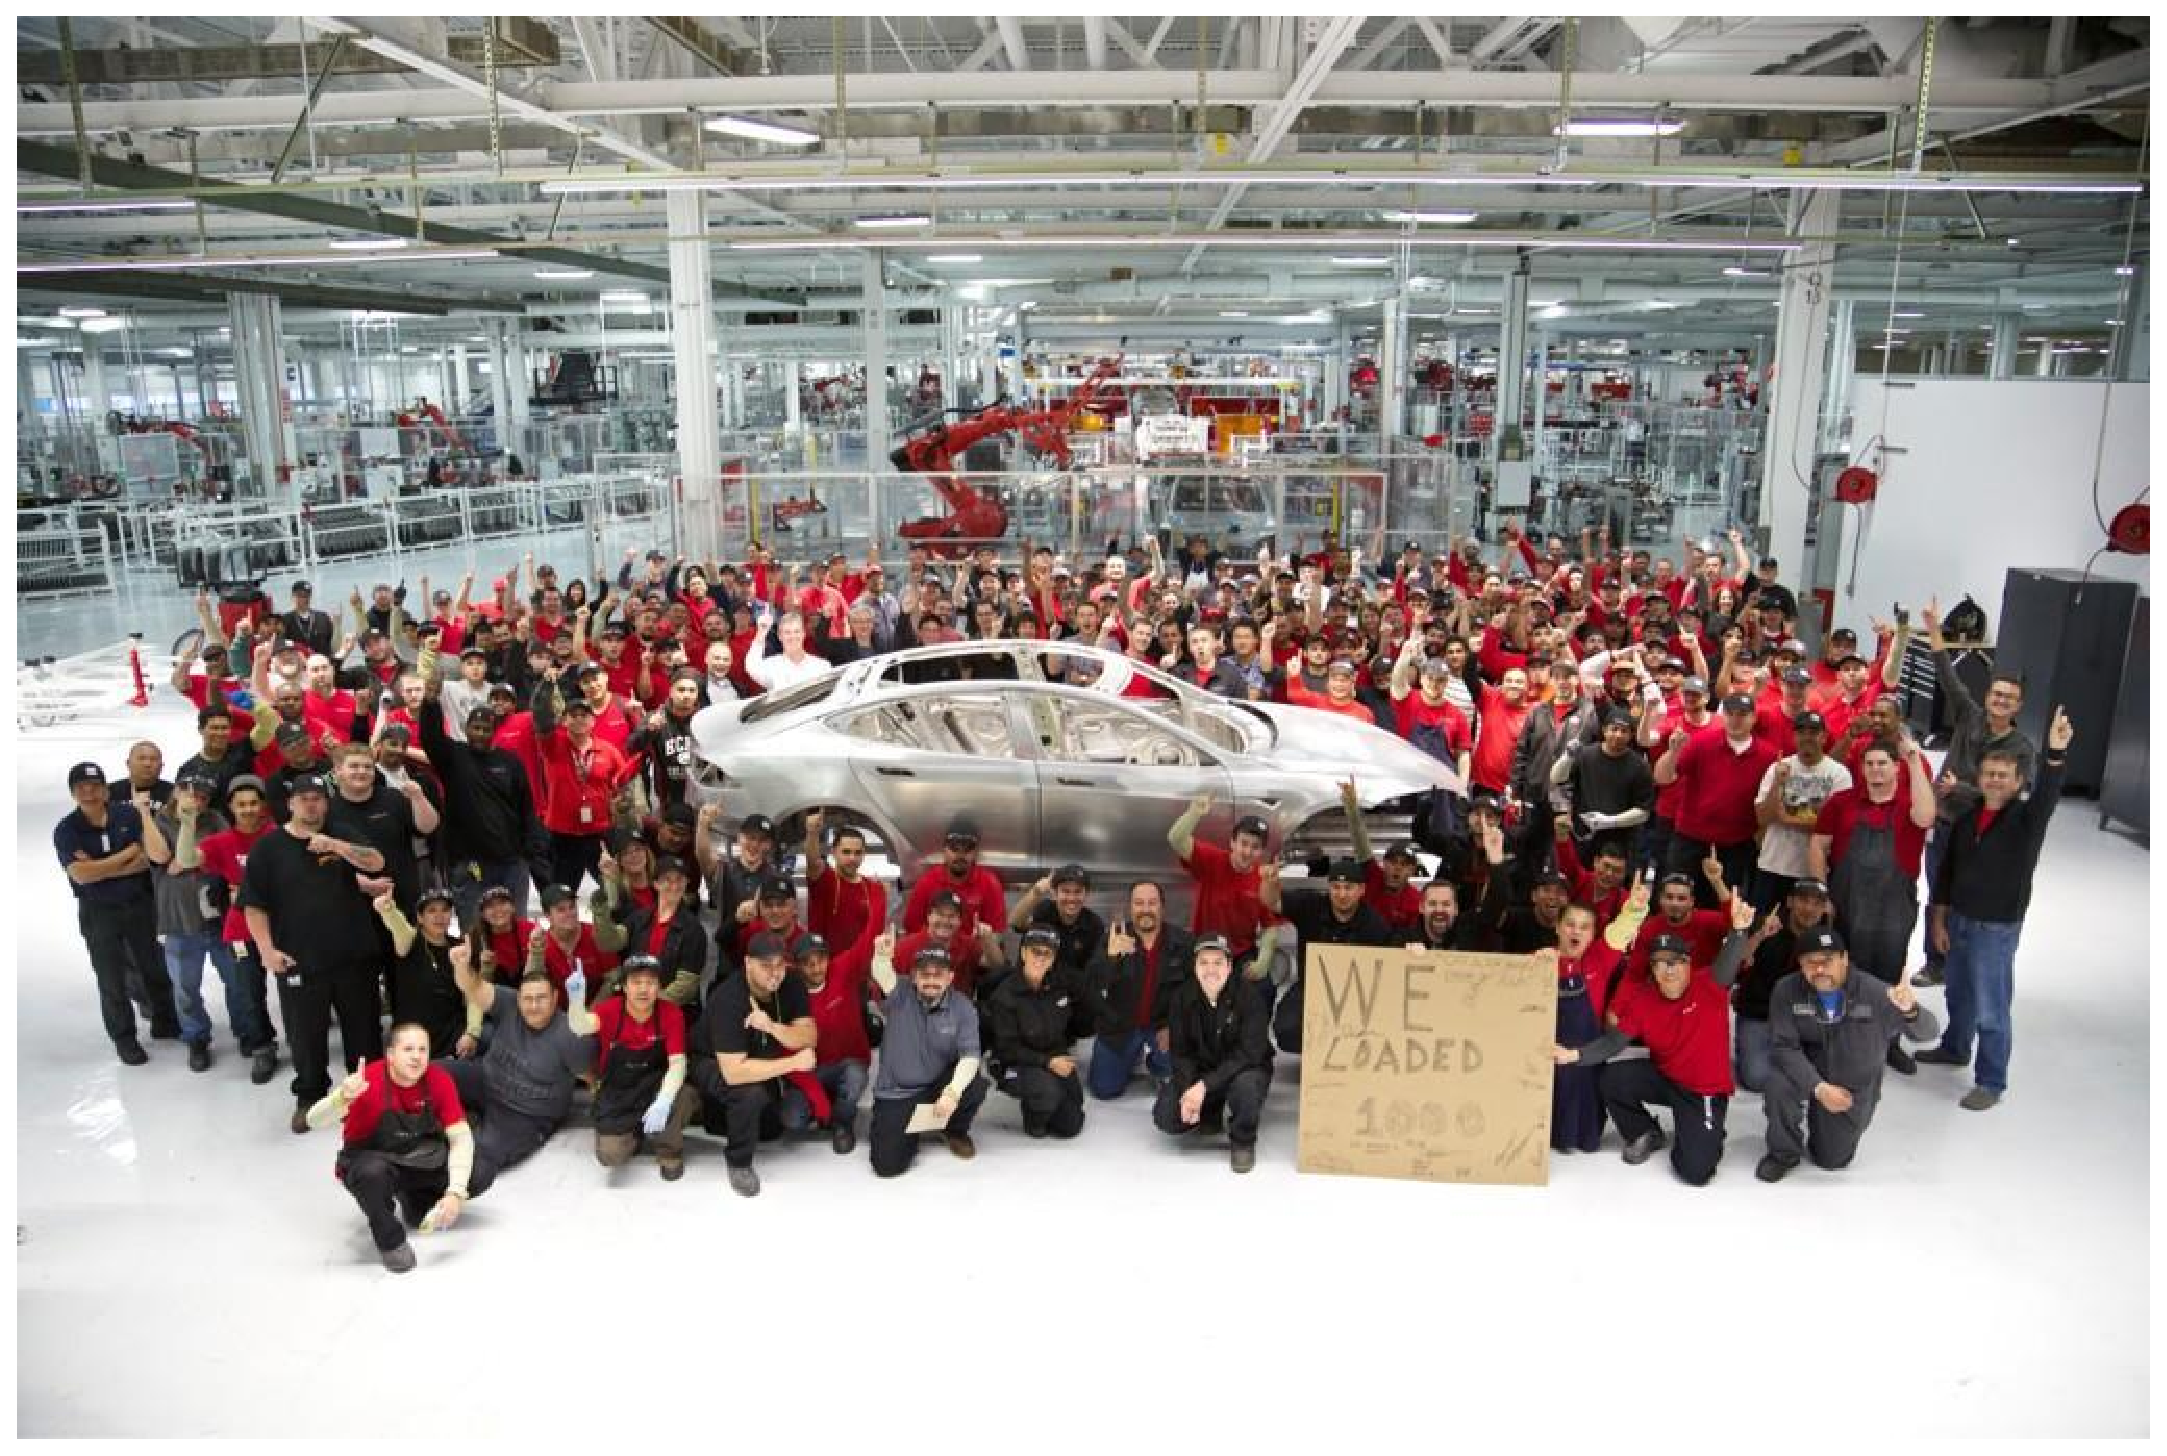
\includegraphics[width=\linewidth]{img/teslateam.eps}
\end{frame}

\begin{frame}
\textbf{Scientific working is a social discipline that includes}
\begin{itemize}
\item Having great ideas
\item Actually doing own research and science
\item Working in the teams
\item Raising money
\item Publishing papers
\item Giving presentations
\item Evaluating others people work
\end{itemize}
\textbf{This class will streghten your skills in}
\begin{itemize}
\item Giving presentations on scientific topics
\item Working in the teams
\item Evaluating others people work
\end{itemize}
\end{frame}

\begin{frame}
\frametitle{Scientists are evaluated based on their publications}
\begin{itemize}
\item Measurement of quality of publication is a impact factor of the journal (IF)
\item One needs to compare journal impact factors within particular field
\item Medical and economical journals tend to have higher impact factors
\item Better journals have more stricter quality standards
\item Higher impacted journals = higher rejection rate (i.e. 70\%)
\item Well established per-rewiew process
\item Experts in the field evaluates work of the scientists
\item \textbf{Accept, change, reject}
\end{itemize}
\end{frame}

\begin{frame}
\frametitle{Survey of the good journals in Medical engineering}
\begin{table}[]
\centering
\label{my-label}
\tiny{\begin{tabular}{@{}lll@{}}
\toprule
\textbf{Journal}                                            & \textbf{Impact Factor} & \textbf{Proposed by}                        \\ \midrule
\textit{Stroke}                                             & 6.032                  & Sebastian Bannasch                          \\
\textit{NeuroImage}                                         & 5.835                  & Domenico Iuso                               \\
\textit{Medical Image Analysis}                             & 4.188                  & Samuel Manthey                              \\
\textit{\textbf{IEEE Transactions on Medical Imaging}}      & \textbf{3.942}         & \textbf{S. Bannasch, S. Manthey, R. Frysch} \\
\textit{American Journal of Neuroradiology}                 & 3.55                   & Sebastian Bannasch                          \\
\textit{Medical Physics}                                    & 2.617                  & Sebastian Bannasch                          \\
\textit{Physics in Medicine \& Biology}                     & 2.742                  & Domenico Iuso, Robert Frysch                \\
\textit{IEEE Signal Processing Letters}                     & 2.528                  & Robert Frysch                               \\
\textit{Int. J. of Computer Assisted Radiology and Surgery} & 1.863                  & Samuel Manthey                              \\ \bottomrule
\end{tabular}}
\end{table}

\footnotesize{
\begin{itemize}
\item Do your own research
\item Ask for a good journals from your field
\item If you would publish your results, what journal you would have choosen?
\end{itemize}
}
\end{frame}

\begin{frame}
\frametitle{Class assignments}
\begin{itemize}
\item You will learn how to interact in the peer review process
\item You will form 3 people committees that resemble journal boards
\item Committees specify their specific interests
\item Committees will offer papers in their field for presentation
\item OVGU Ph.D. students suggested some papers, see course webpages
\item You will apply to a commitee for presentation
\item You will review proposals of other presentations
\item You will improve your presentation based on the reviews and deliver it in class
\end{itemize}
\end{frame}
